\documentclass[10pt,a4paper,final]{article}
\usepackage[utf8]{inputenc}
\usepackage[francais]{babel}
\usepackage[T1]{fontenc}
\usepackage{amsmath}
\usepackage{amsfonts}
\usepackage{graphicx}
\usepackage{amssymb}
\usepackage{lmodern}
\usepackage[table,xcdraw]{xcolor}
\author{Òsca-Font dubèrta}
\thispagestyle{empty}

\begin{document}


\begin{center}

\includegraphics[height=50pt]{/usr/local/www/drupal7/sites/default/modules/conjoc/cache/verboc_oc.eps}
\end{center}

\begin{center}
\huge{Conjugador lengadocian}
\end{center}

\section*{crestar_2}
\subsection*{Modèl «110»}
\subsection*{conjugason 1 alternant è/e}
\begin{tabular}{|c|c|c|c|c|}
\hline 
\multicolumn{5}{|c|}{\textbf{Infinitiu}} \\ 
\hline 
 & \textbf{Present} & \textbf{Imperfach} & \textbf{Preterit} & \textbf{Futur} \\ 
\hline 
\textit{s1} & crèsti & crestavi & crestèri & crestarai \\ 
\hline 
\textit{s2} & crèstas & crestavas & crestères & crestaràs \\ 
\hline 
\textit{s3} & crèsta & crestava & crestèt & crestarà \\ 
\hline 
\textit{s1} & crestam & crestàvem & crestèrem & crestarem \\ 
\hline 
\textit{s2} & crestatz & crestàvetz & crestèretz & crestaretz \\ 
\hline 
\textit{s3} & crèstan & crestavan & crestèron & crestaràn \\ 
\hline 
\multicolumn{5}{|c|}{} \\ 
\hline 
 & \multicolumn{2}{c|}{\textbf{Subjontiu}}  & \multicolumn{2}{c|}{\textbf{Imperatiu}} \\ 
\hline 
 & \textbf{Present} & \textbf{Imperfach} & \textbf{Forma affirmativa} & \textbf{Forma negativa} \\ 
\hline 
\textit{s1} & crèste & crestèsse & \multicolumn{2}{c|}{} \\ 
\hline 
\textit{s2} & crèstes & crestèsses & crèsta & crèstes \\ 
\hline 
\textit{s3} & crèste & crestèsse & \multicolumn{2}{c|}{} \\ 
\hline 
\textit{p1} & crestem & crestèssem & crestem & crestem \\ 
\hline 
\textit{p2} & crestetz & crestèssetz & crestatz & crestetz \\ 
\hline 
\textit{p3} & crèsten & crestèsson & \multicolumn{2}{c|}{} \\ 
\hline 
\multicolumn{5}{|c|}{} \\ 
\hline 
 & \multicolumn{2}{c|}{\textbf{Conditional}} & \multicolumn{2}{c|}{} \\ 
\hline 
 &  \multicolumn{2}{c|}{\textbf{Present}} & \multicolumn{2}{c|}{\textbf{Formas impersonalas}}  \\ 
\hline 
\textit{s1} & \multicolumn{2}{c|}{crestariái}  & \textbf{Infinitiu} & crestar \\ 
\hline 
\textit{s2} & \multicolumn{2}{c|}{crestariás}  & \textbf{Gerondiu} & crestant \\ 
\hline 
\textit{s3} & \multicolumn{2}{c|}{crestariá}  & \textbf{Participi passat} & crestat / crestada \\ 
\hline 
\textit{p1} & \multicolumn{2}{c|}{crestariam} & \multicolumn{2}{c|}{} \\ 
\hline 
\textit{p2} & \multicolumn{2}{c|}{crestariatz} & \multicolumn{2}{c|}{} \\ 
\hline 
\textit{p3} & \multicolumn{2}{c|}{crestarián} & \multicolumn{2}{c|}{} \\ 
\hline 
\end{tabular}

\begin{center}

\includegraphics[width=100pt]{/usr/local/www/drupal7/sites/default/modules/conjoc/cache/logoCongres300.jpg}
\end{center}

\hfill\includegraphics[width=40pt]{/usr/local/www/drupal7/sites/default/modules/conjoc/cache/by-sa.eps}

\end{document}
